
\section{The Yeh--Petroff dam break problem}
Yeh and Petroff of the University of Washington conducted experimental dam break with an obstruction column, as shown in Figure~\ref{fig:YP}.
The Yeh--Petroff dam break problem was further simulated by Gomez-Gesteira and Dalrymple~\cite{GD2004} and Silvester and Cleary~\cite{SC2006}. A similar problem was studied by Arnason et al.~\cite{APY2009}.
We shall compare our \anuga{} solution to the experimental data of Yeh and Petroff.

\begin{figure}
\begin{center}
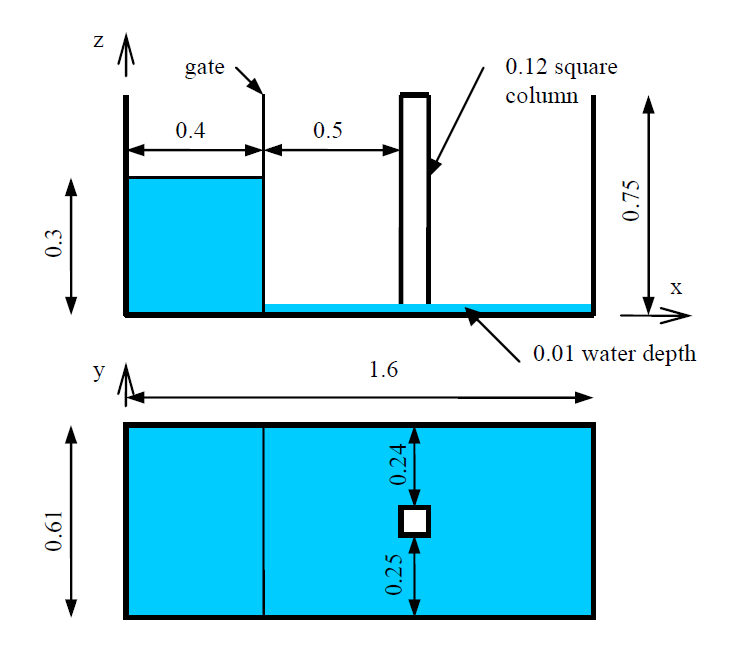
\includegraphics[width=0.9\textwidth]{Yeh_Petroff.png}
\end{center}
\caption{Schematic diagram of the inital condition and geometry of the Yeh--Petroff dam break problem (source: Silvester and Cleary~\cite{SC2006}.)} \label{fig:YP}
\end{figure}




\subsection{Results}

We should see excellent agreement between the experimental data and the numerical solution. 

\begin{figure}
\begin{center}
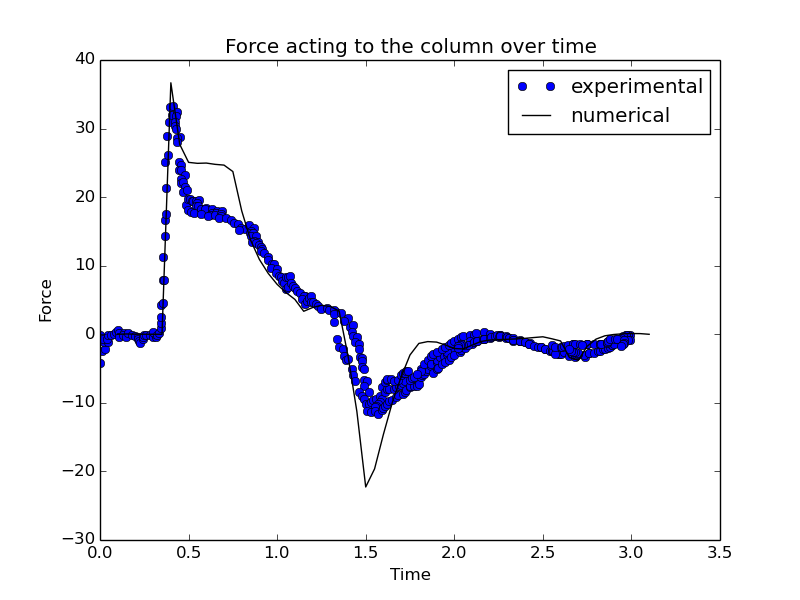
\includegraphics[width=0.9\textwidth]{force.png}
\end{center}
\caption{Stage results}
\end{figure}
%
%
%\begin{figure}
%\begin{center}
%\includegraphics[width=0.9\textwidth]{xmom_plot.png}
%\end{center}
%\caption{Xmomentum results}
%\end{figure}
%
%
%\begin{figure}
%\begin{center}
%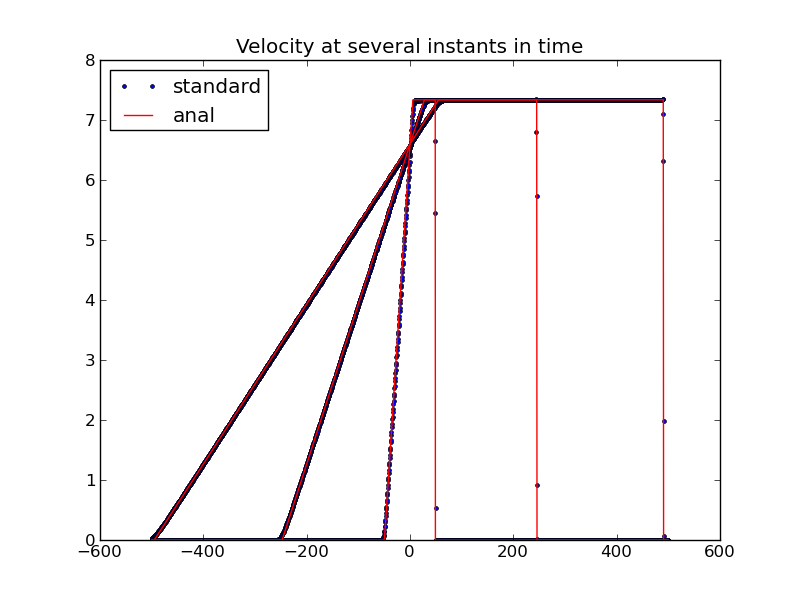
\includegraphics[width=0.9\textwidth]{xvel_plot.png}
%\end{center}
%\caption{Xvelocity results}
%\end{figure}


\endinput
